
\subsection{Analyse Sparkasse}
Die Sparkasse hat in der Entwicklung ihrer Startseite auch React und MUI verwendet. Deshalb ist eine Betrachtung dieser Seite besonders wertvoll. 

Die Startseite weist eine geringe Anzahl an Fehlern auf. Ein Fehler tritt aber wiederholt auf. Dabei handelt es sich um einen Verstoß gegen Kriterium 1.3.1 "Info und Beziehungen". Konkret werden Listenelemente \lstinline{<li>} nicht korrekt in einer Liste \lstinline{<ul>} oder \lstinline{<ol>} verwendet. Dabei ist das HTML-Element mit \lstinline{<li>} richtig angelegt, aber als role wurde article verwendet. Somit wird die Liste nicht korrekt interpretiert.

\begin{figure}[H]
    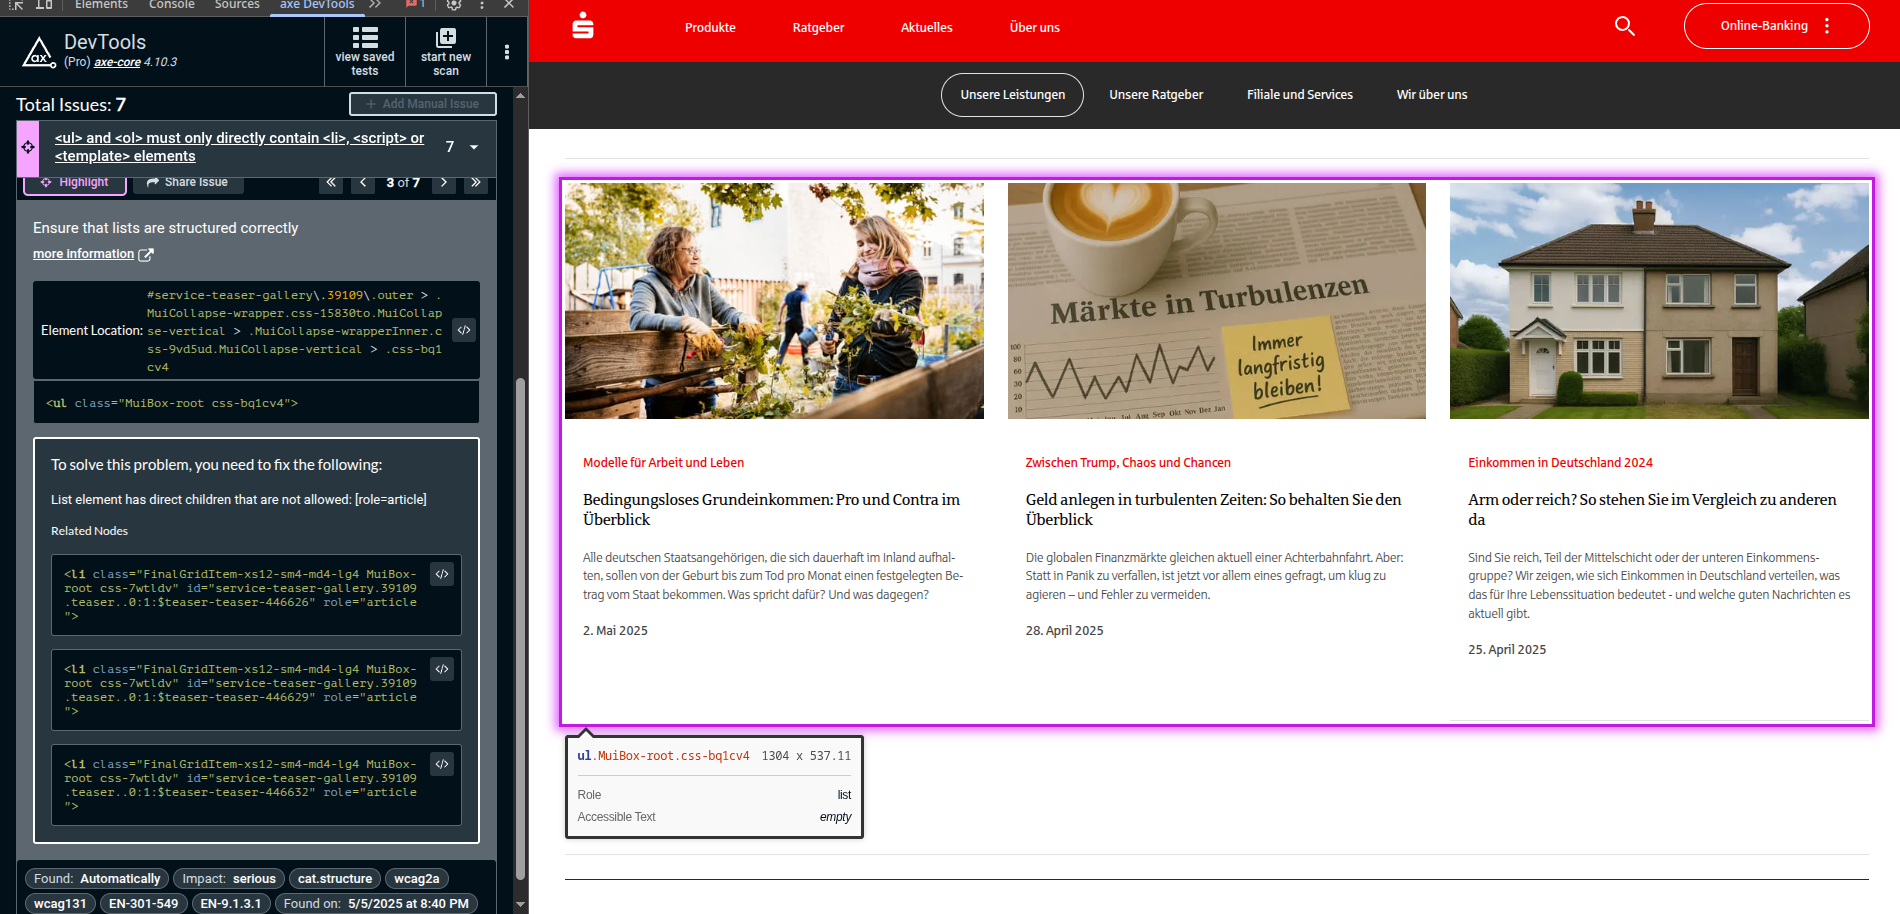
\includegraphics[width=\textwidth]{img/sparkasse_ul-li-wrong-role.png}
    \caption{Fehlerhafte Verwendung von Listen-Elementen}
\end{figure}

Manche Fehler betreffen auch gleich mehrere Regeln. So wurde von WAVE festgestellt, dass es kein Label bei einem Suchfeld gibt. Dies verstößt gleich gegen 4 WCAG-Kriterien 1.1.1 "Nicht-Text-Inhalt", 1.3.1 "Info und Beziehungen", 2.4.6 "Überschriften und Beschriftungen" und 3.3.2 "Labels oder Anleitungen".

\begin{figure}[H]
    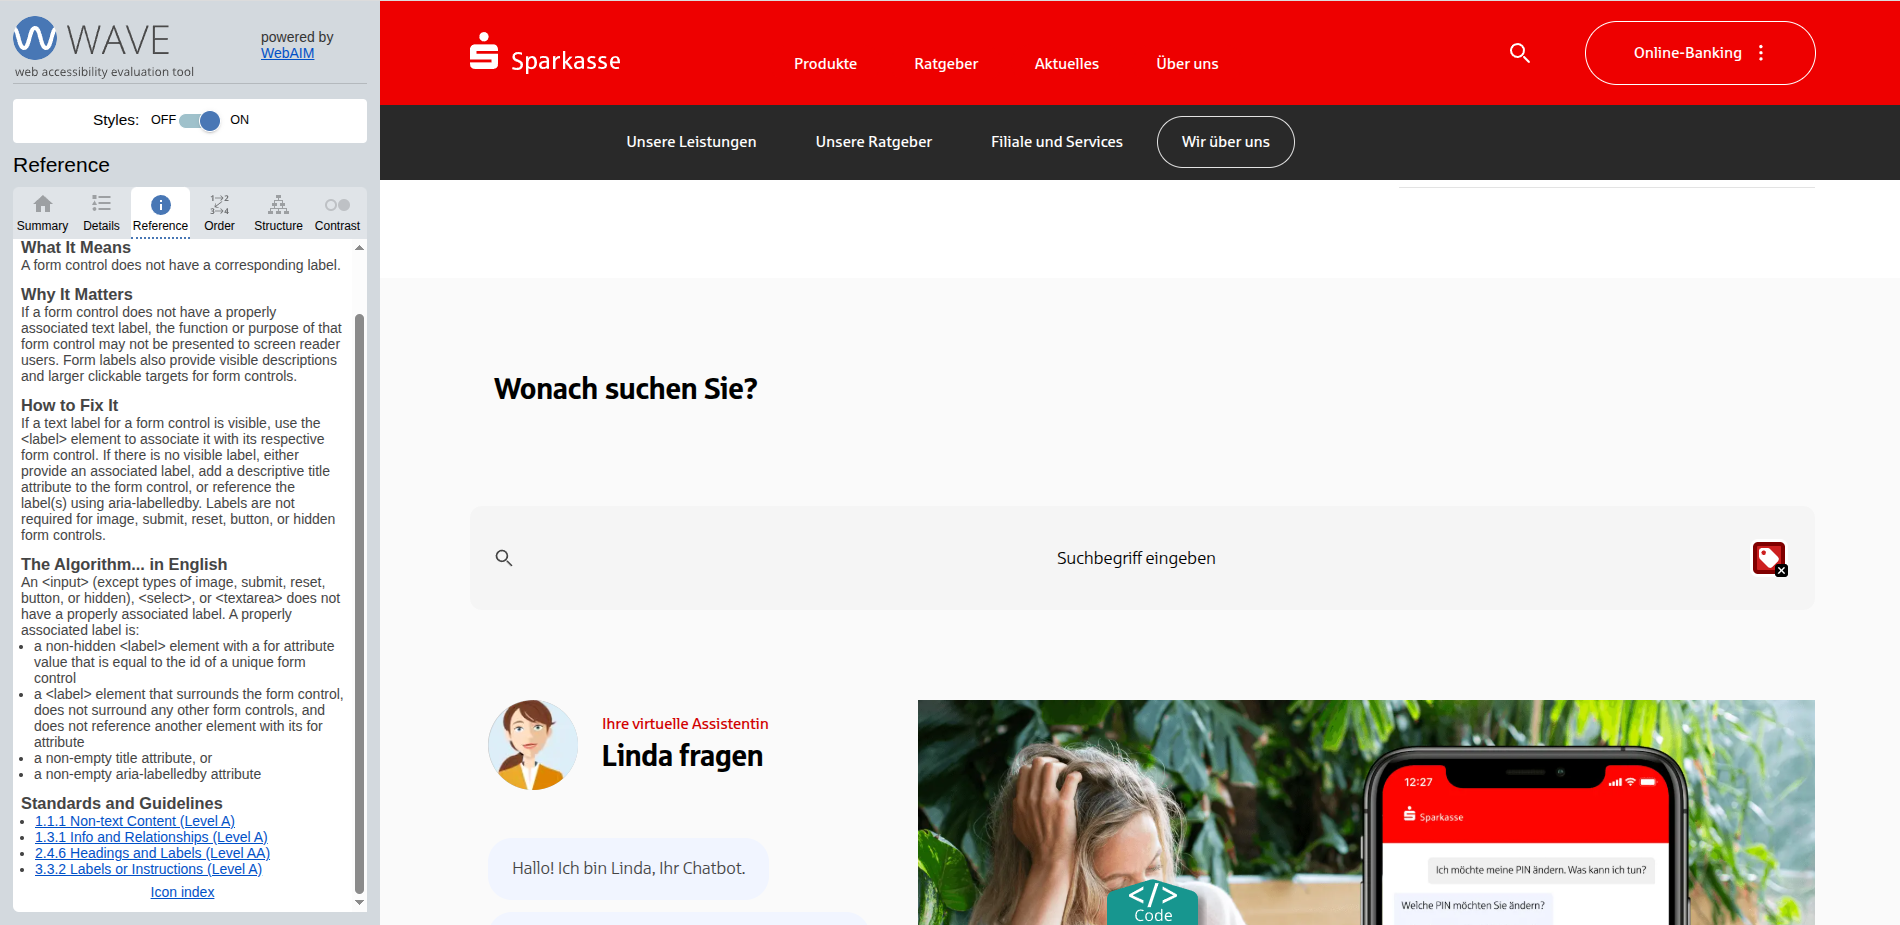
\includegraphics[width=\textwidth]{img/sparkasse_no-label.png}
    \caption{Fehlendes Label bei einem Suchfeld}
\end{figure}

\begin{figure}[H]
    \begin{tikzpicture}
        \begin{axis}[
            width=\textwidth,
            height=10cm,
            ybar,
            bar width=12pt,
            xlabel={WCAG-Kriterium},
            ylabel={Fehleranzahl},
            symbolic x coords={ 9.1.1.1, 9.1.3.1, 9.2.4.4, 9.2.4.6, 9.2.4.7, 9.3.3.2, 9.4.1.2 },
            xtick=data,
            x tick label style={rotate=45, anchor=east},
            ymin=0,
            ymax=300,
            enlarge x limits=0.1,
            legend style={cells={anchor=west}, legend pos=north east},
            nodes near coords,
            nodes near coords style={font=\scriptsize},
        ]
            \addplot table[x=WCAG-Kriterium,y=Fehleranzahl_axe,col sep=tab] {csv/output/wcag_analyse_sparkasse_xxxx.csv};
            \addplot table[x=WCAG-Kriterium,y=Fehleranzahl_WAVE,col sep=tab] {csv/output/wcag_analyse_sparkasse_xxxx.csv};
            \legend{axe,WAVE}
        \end{axis}
    \end{tikzpicture}
    \caption{Auswertung Analyse Sparkasse}
\end{figure}
